
\subheading{16. APPENDIX}\par
\subheading{16.1 SCREENSHOTS}

\noindent \textbf{Login page}\nopagebreak\par
\vspace{0.2cm}\nopagebreak
\noindent 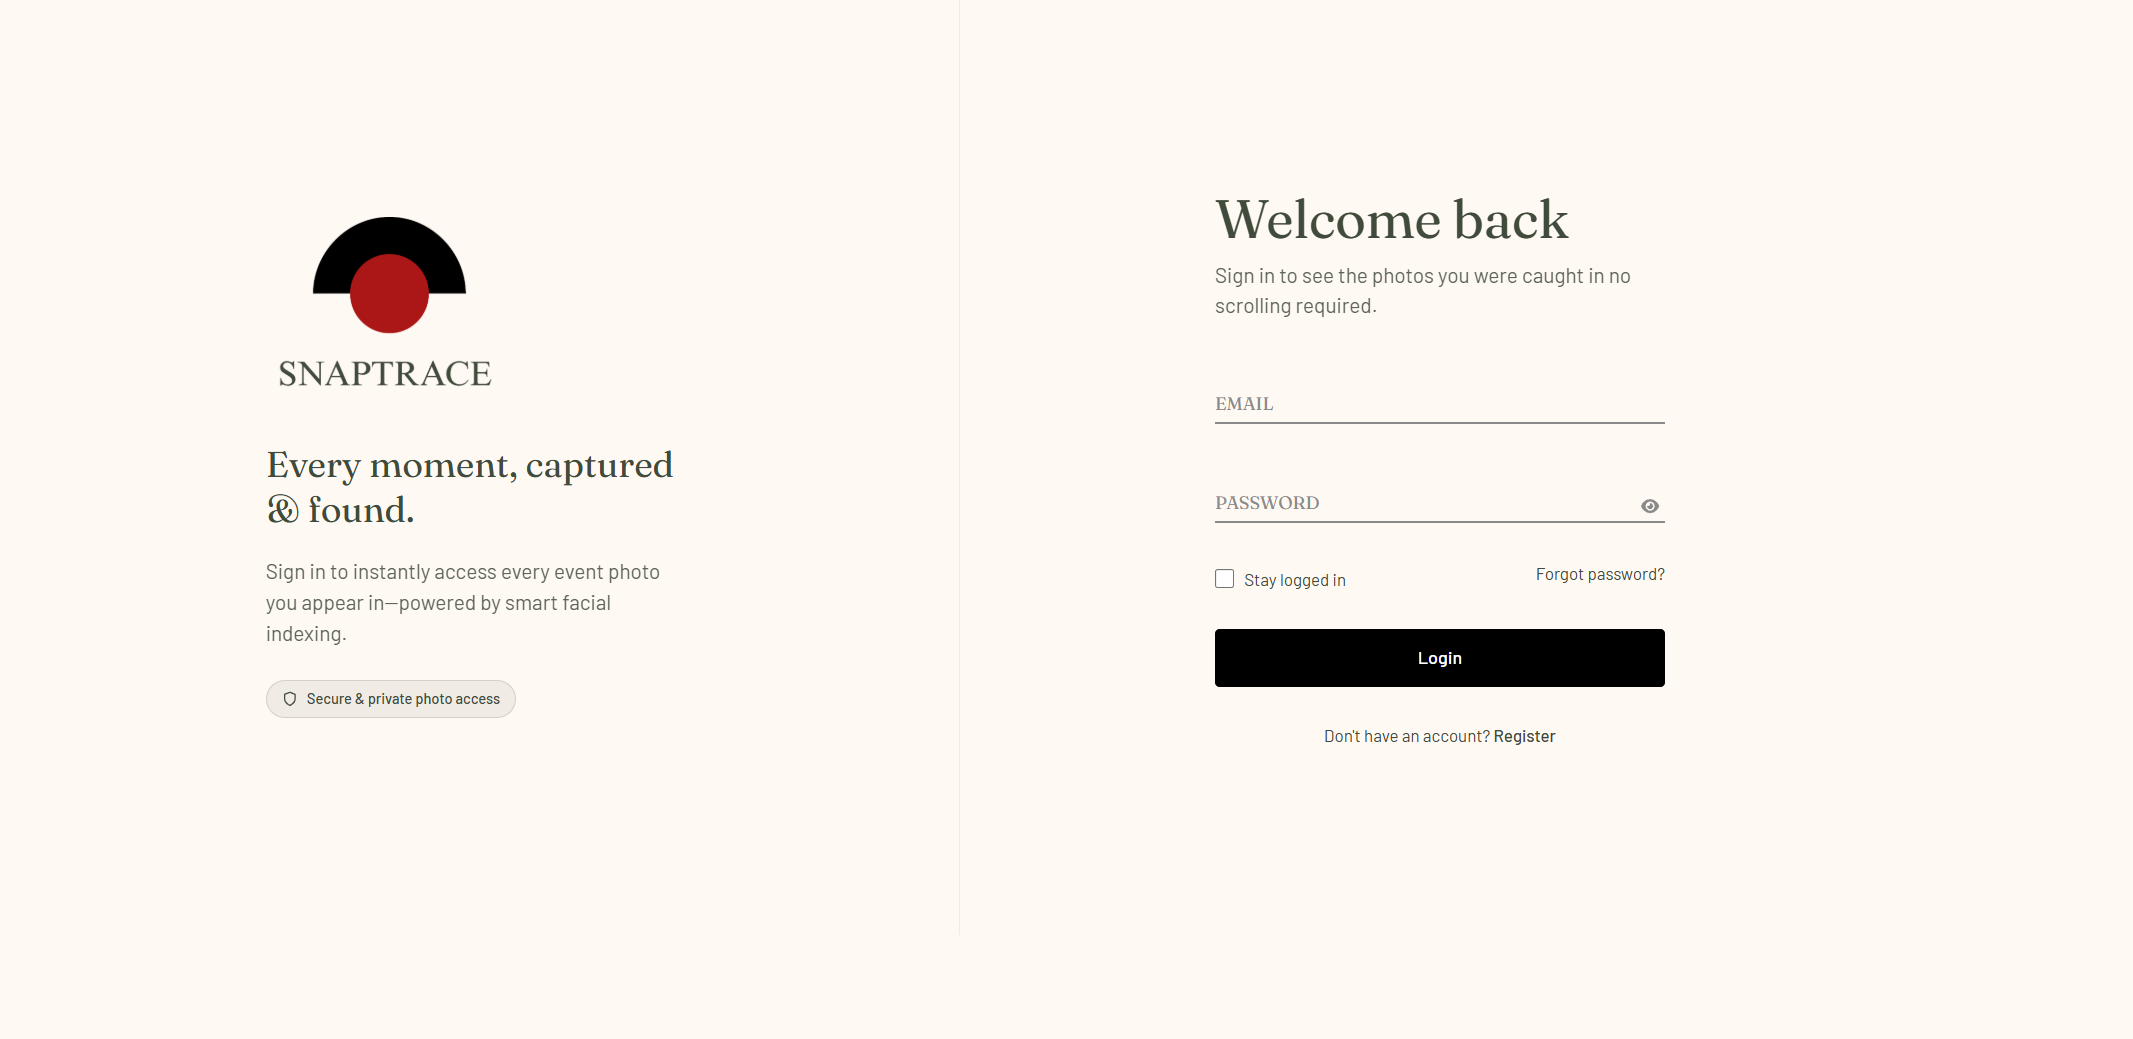
\includegraphics[width=1\textwidth]{screenshot/loginPage.png}\par
\vspace{0.5cm}

\noindent \textbf{Register Page}\nopagebreak\par
\vspace{0.2cm}\nopagebreak
\noindent 
\includegraphics[width=1\textwidth]{screenshot/registerpage.png}\par
\vspace{0.5cm}

\noindent \textbf{Home Page}\nopagebreak\par
\vspace{0.2cm}\nopagebreak

\includegraphics[width=15cm, height=22cm]{screenshot/homepage.png}\par
\vspace{0.5cm}


\noindent \textbf{Face scan}\nopagebreak\par
\vspace{0.2cm}\nopagebreak
\noindent 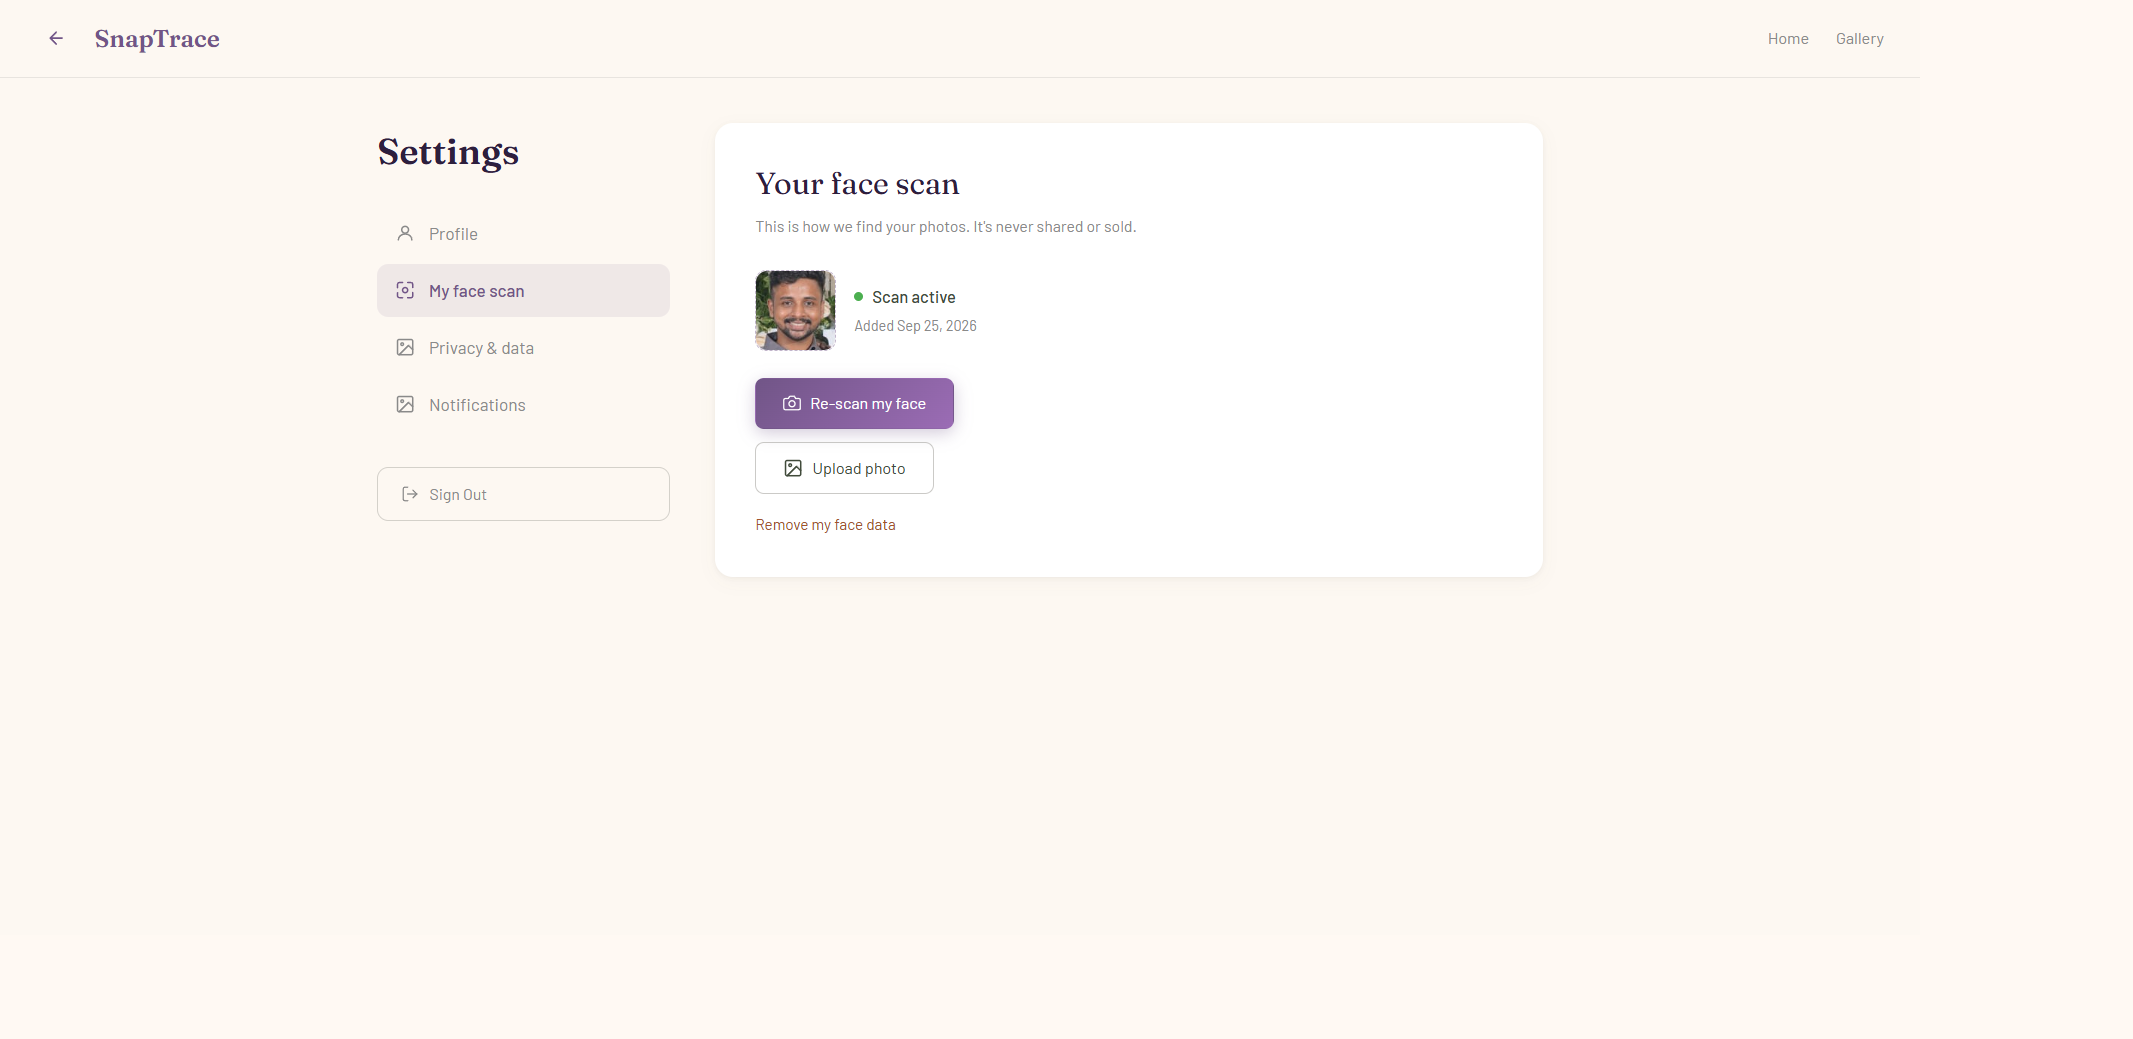
\includegraphics[width=1\textwidth]{screenshot/scanFace.png}\par
\vspace{0.5cm}

\noindent \textbf{Forgot your password}\nopagebreak\par
\vspace{0.2cm}\nopagebreak
\noindent 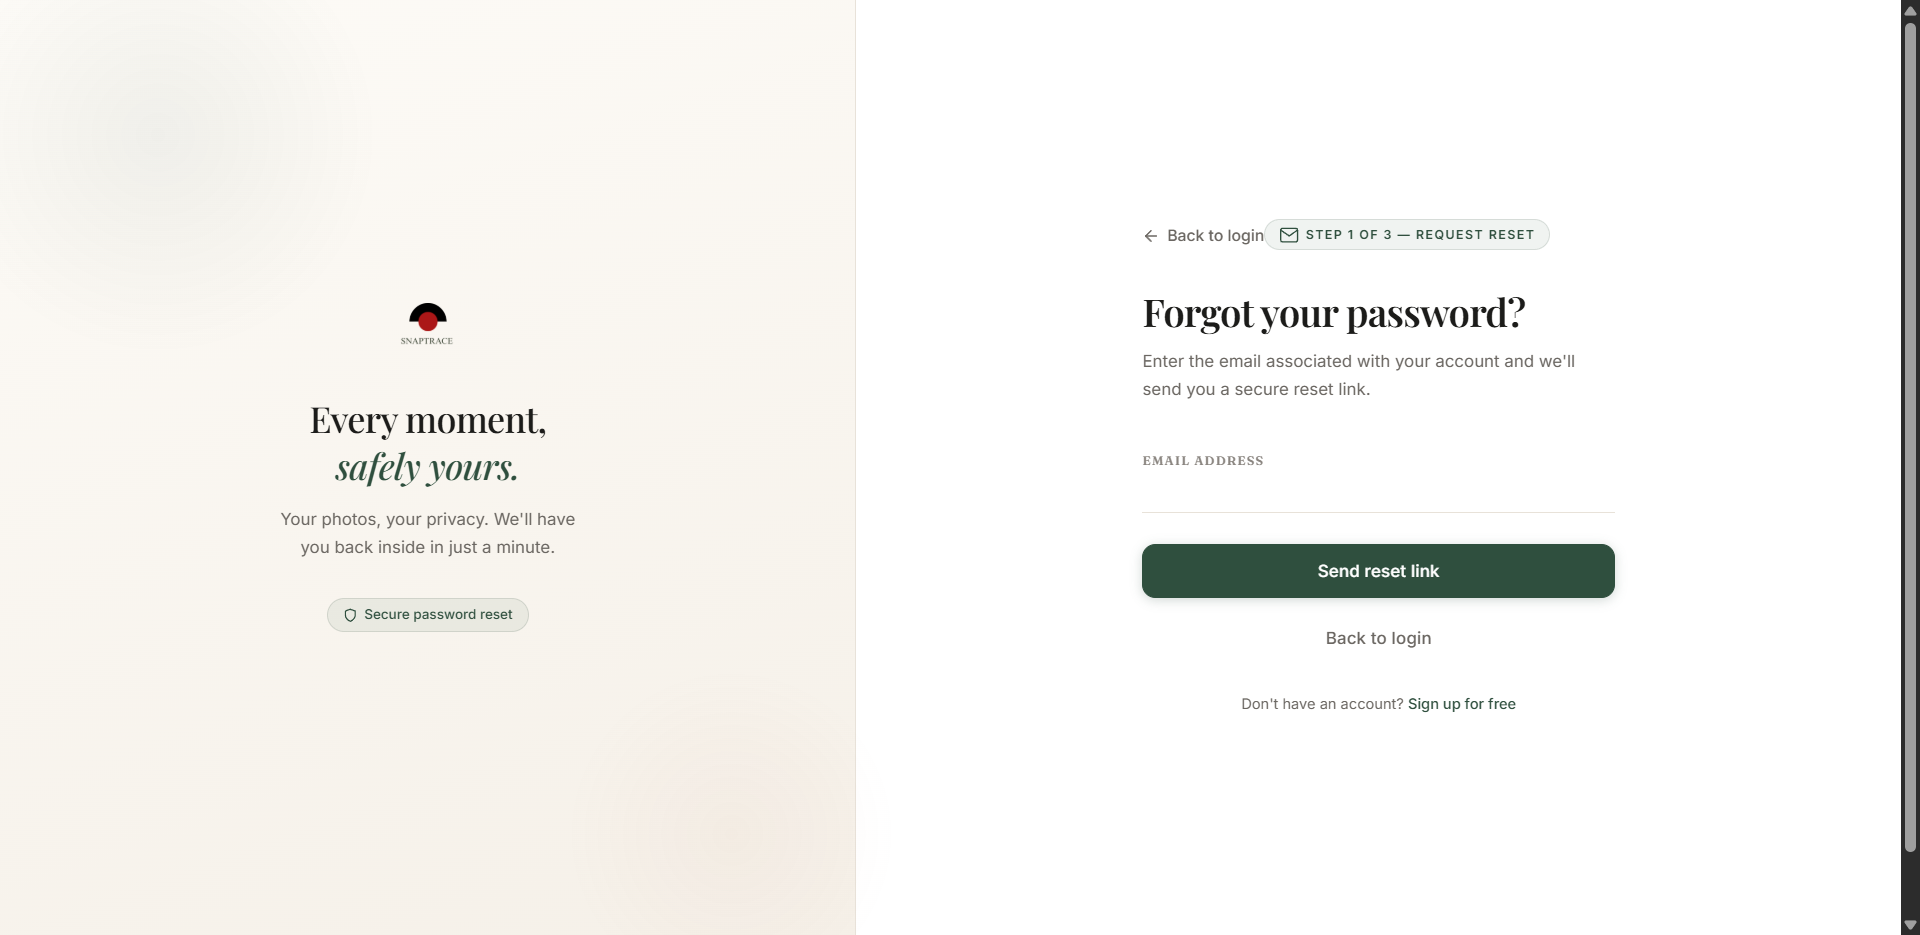
\includegraphics[width=1\textwidth]{screenshot/forgotpage.png}\par
\vspace{0.5cm}

\noindent \textbf{Admin - dashboard}\nopagebreak\par
\vspace{0.2cm}\nopagebreak
\noindent 
\includegraphics[width=1\textwidth]{screenshot/admin dashboard.png}\par
\vspace{0.5cm}

\noindent \textbf{Admin - user management}\nopagebreak\par
\vspace{0.2cm}\nopagebreak
\noindent 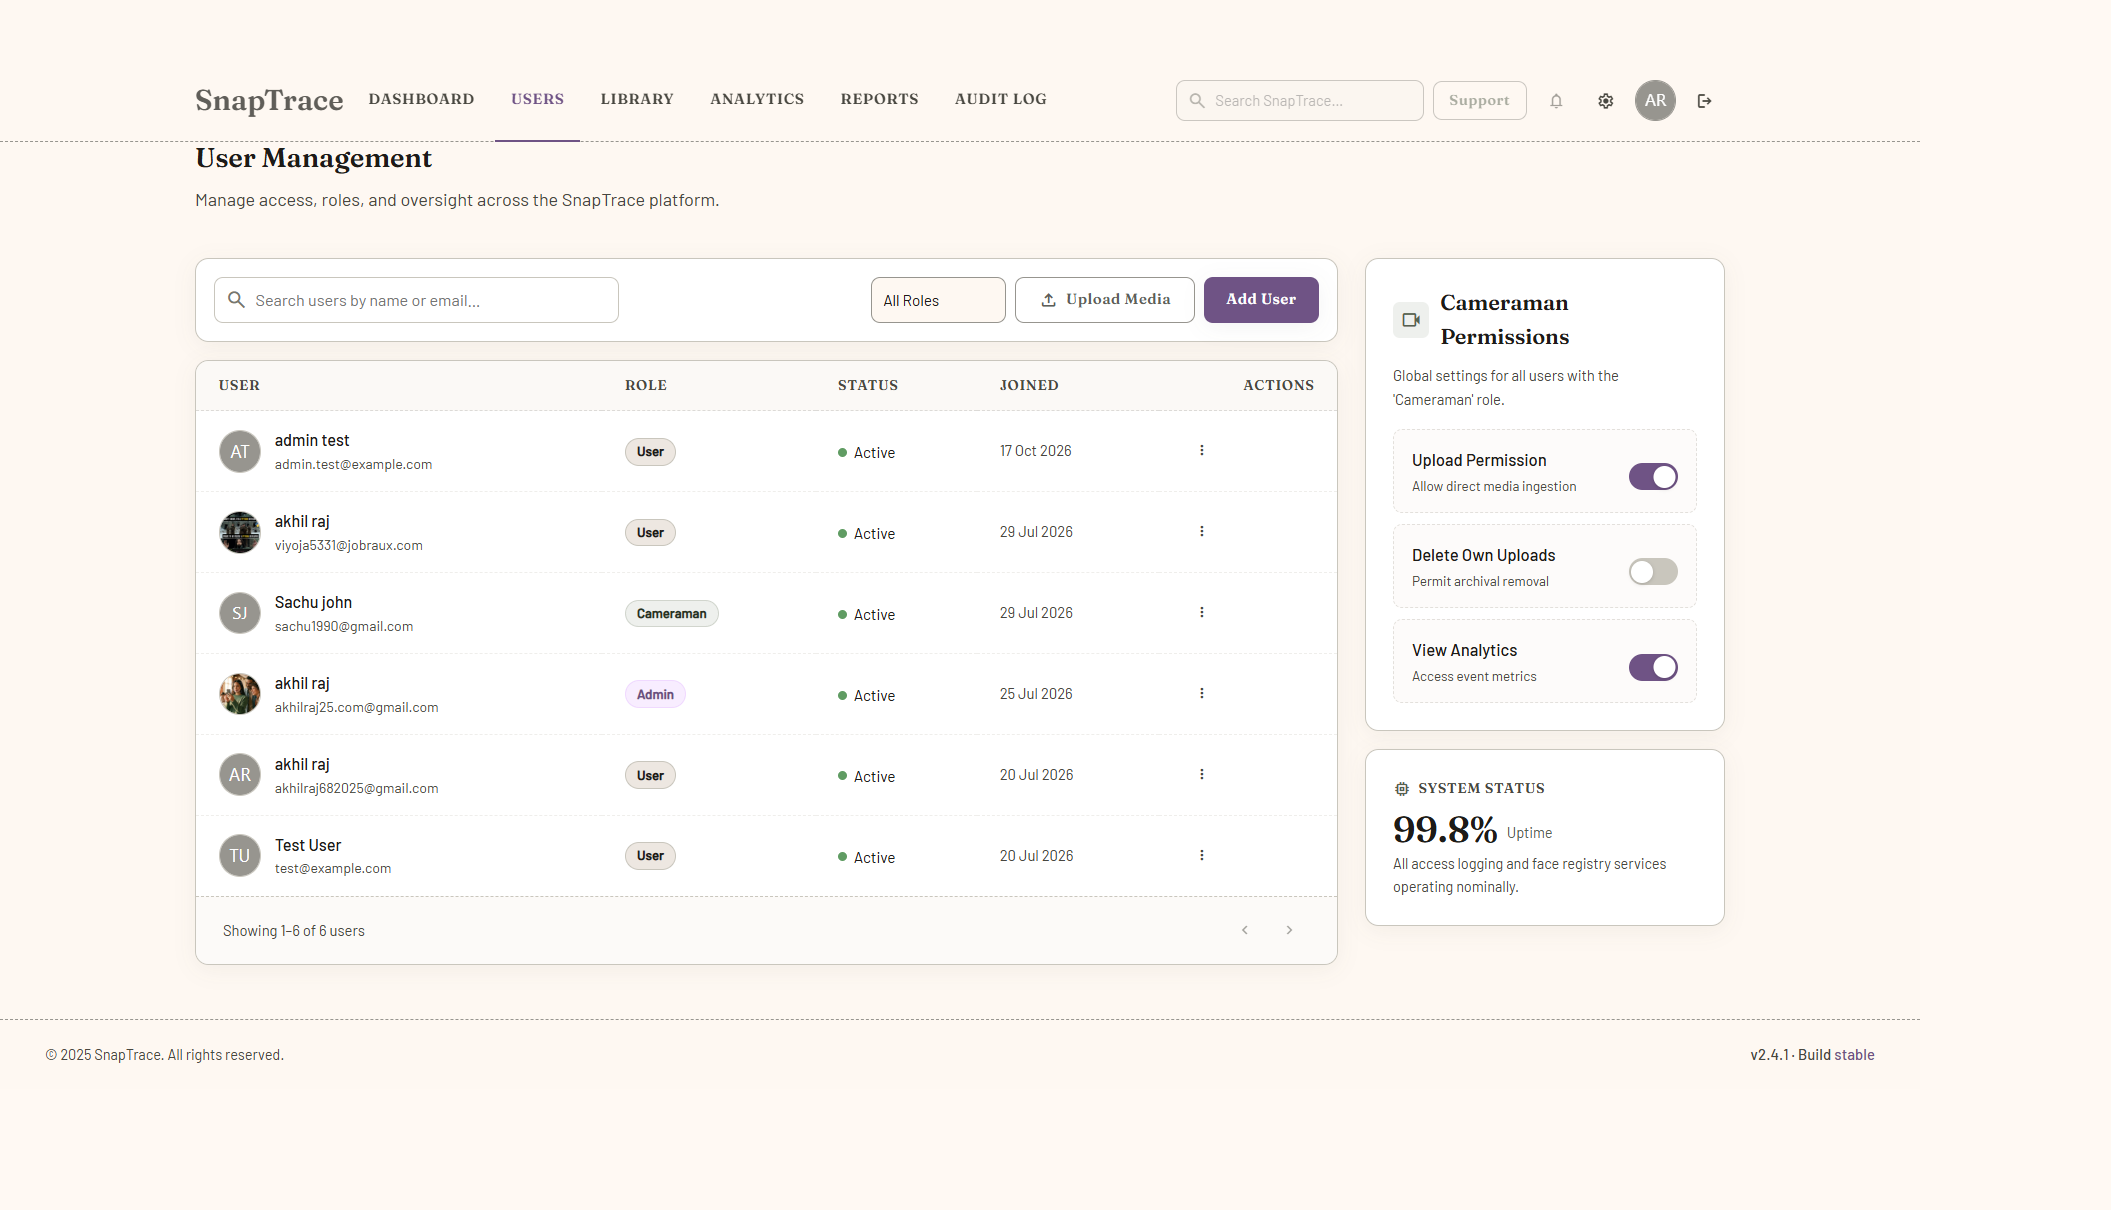
\includegraphics[width=1\textwidth]{screenshot/admin2.png}\par
\vspace{0.5cm}

\noindent \textbf{Admin - Audit log}\nopagebreak\par
\vspace{0.2cm}\nopagebreak
\noindent 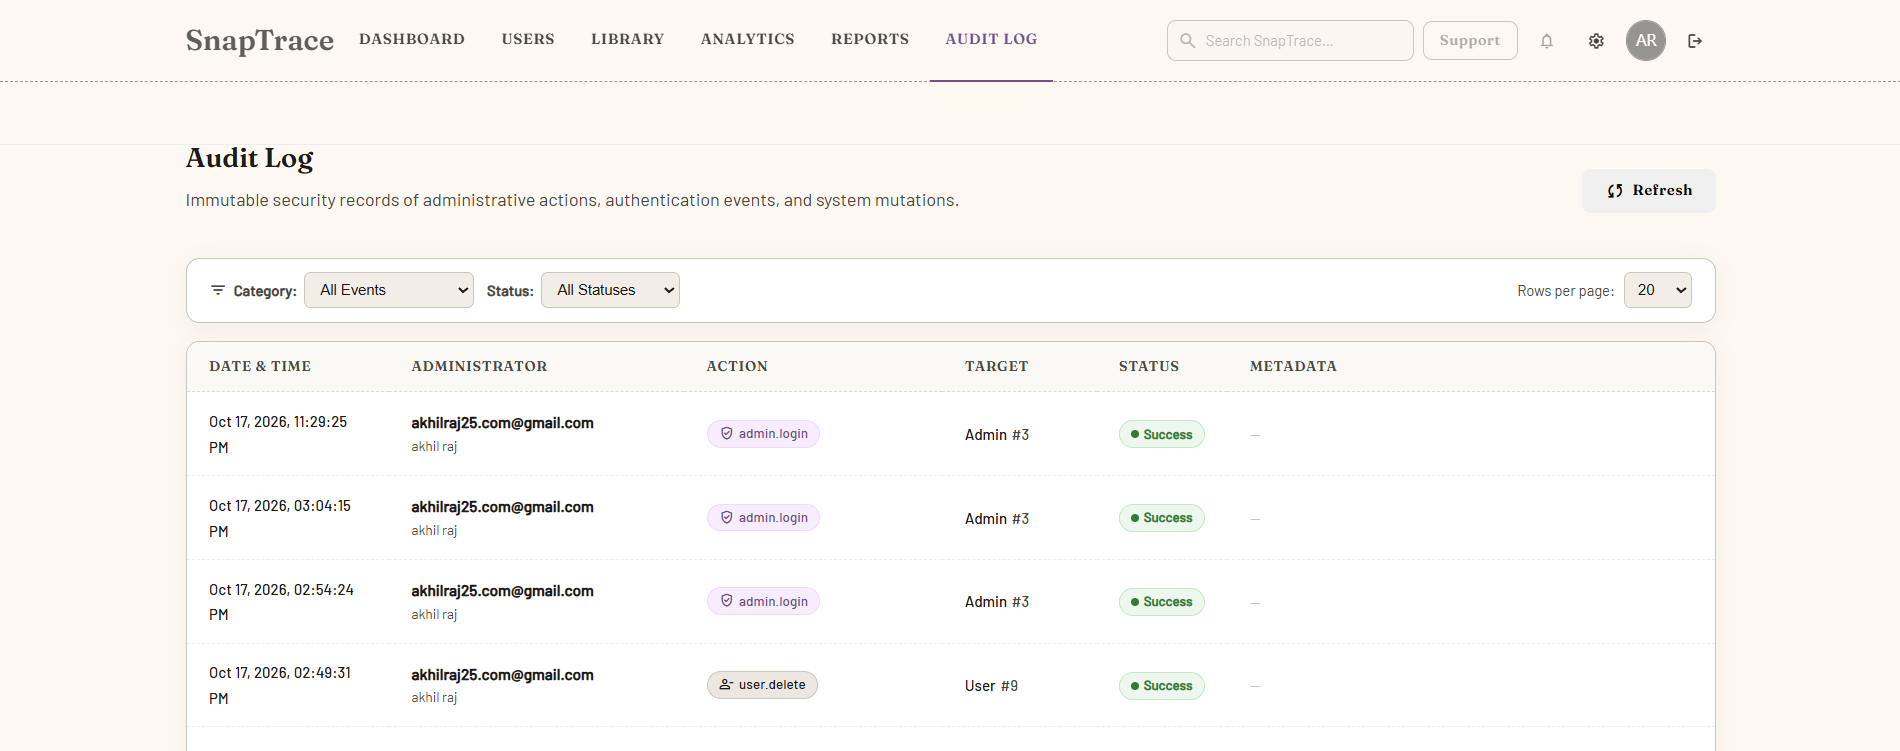
\includegraphics[width=1\textwidth]{screenshot/admin3.png}\par
\vspace{0.5cm}



\noindent \textbf{Cameraman - uploading page}\nopagebreak\par
\vspace{0.2cm}\nopagebreak
\noindent 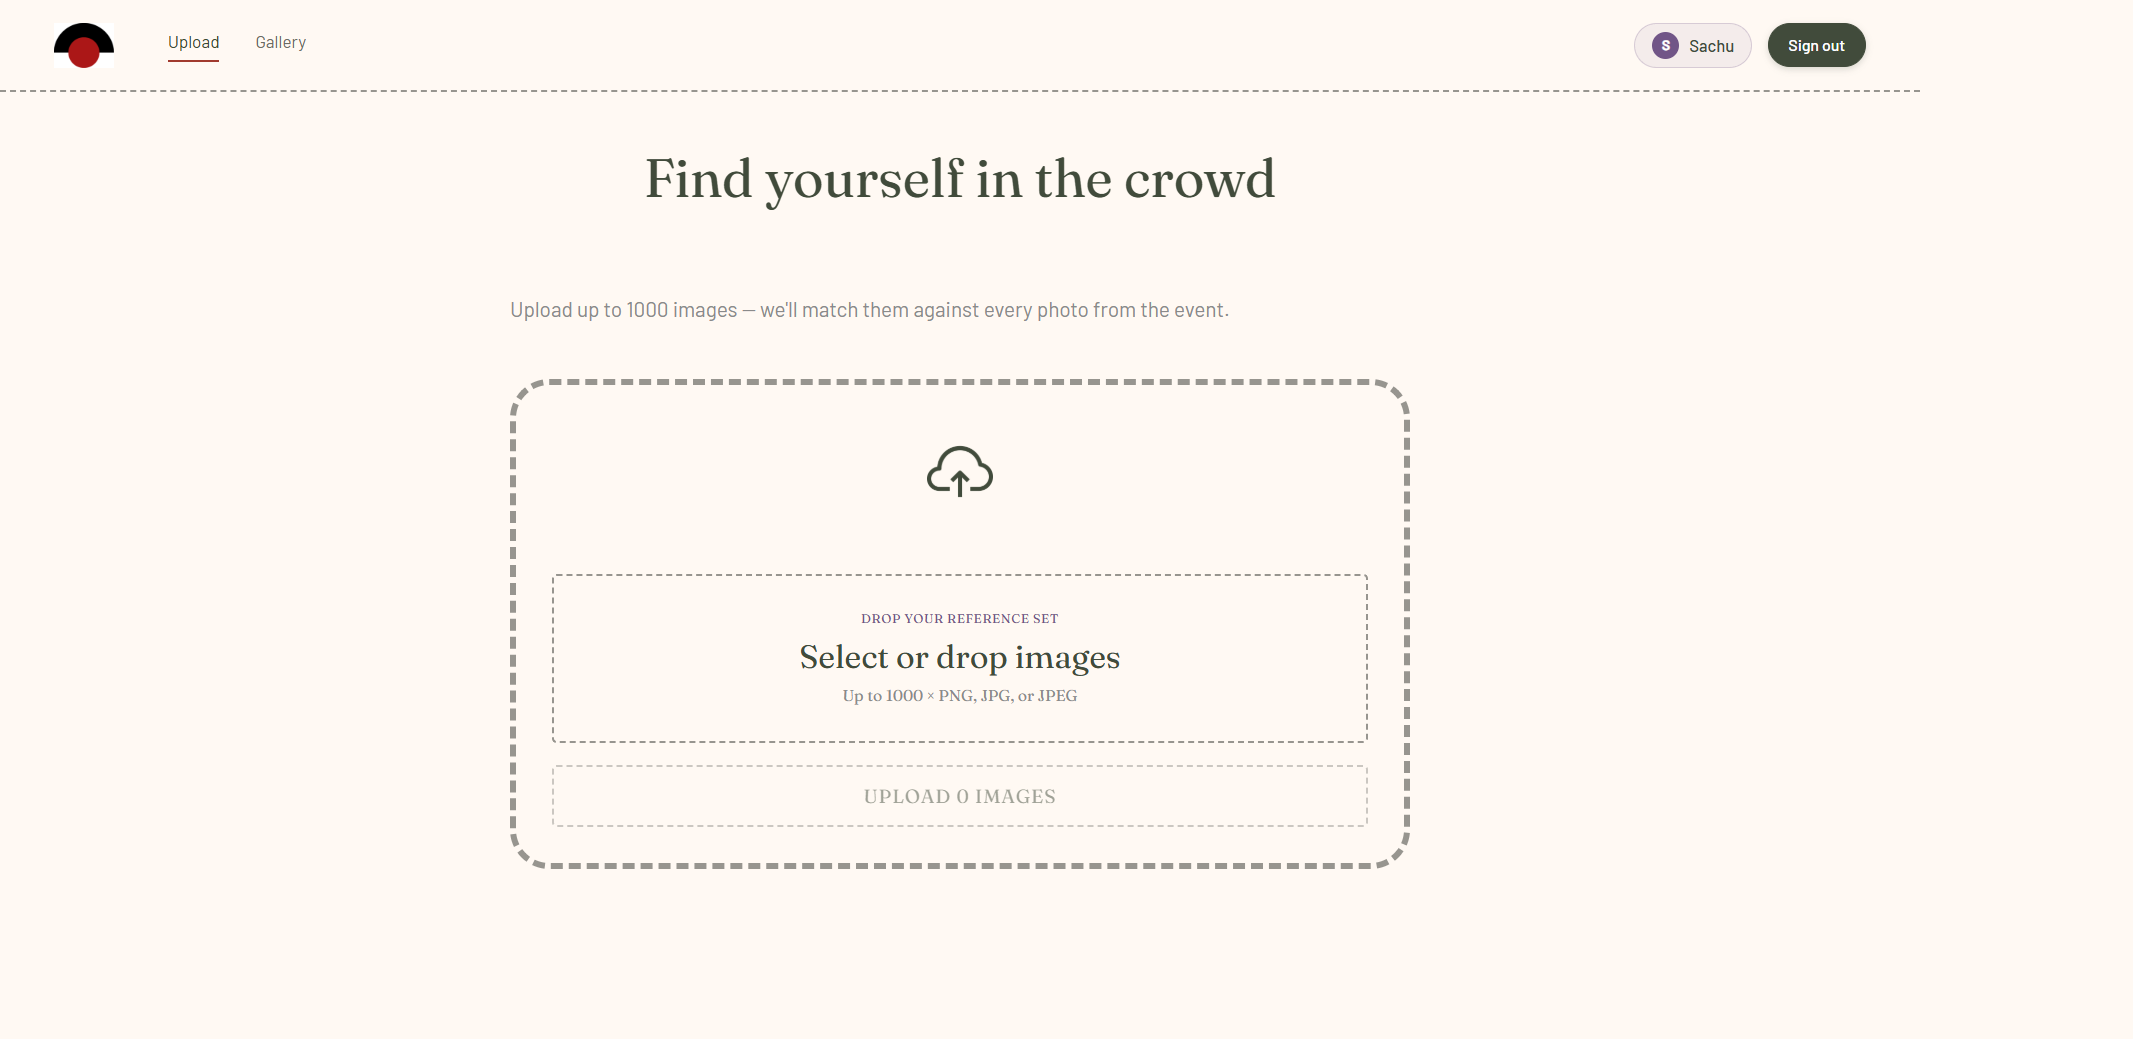
\includegraphics[width=1\textwidth]{screenshot/cameriaMan.png}\par
\vspace{0.5cm}

\clearpage
\subheading{16.2 SOURCE CODE}

\subheading{Frontend Component: \text{src/LoginForm/LoginForm.jsx}}

\begin{lstlisting}[language=JavaScript,frame=none]
import { useState } from 'react';
import { Navigate, useLocation } from 'react-router-dom';
import { loginUser } from '../api/auth';
import { useAuth } from '../context/AuthContext';
import DirectionalTransition from '../components/DirectionalTransition';
import { useTransitionNavigate } from '../hooks/useTransitionNavigate';
import TransitionLink from '../components/TransitionLink';
import logoImg from '../assets/logo.png';
import './Loginform.css';
import Input from '../components/Input';

const EMAIL_REGEX = /^[^\s@]+@[^\s@]+\.[^\s@]+$/;

function LoginForm() {
    const [email, setEmail] = useState('');
    const [password, setPassword] = useState('');
    const [stayLoggedIn, setStayLoggedIn] = useState(false);
    const location = useLocation();
    const navigate = useTransitionNavigate();
    const [loading, setLoading] = useState(false);
    const [error, setError] = useState('');
    const { login, user, loading: authLoading } = useAuth();

    if (!authLoading && user) {
        if (user.role === 'admin') return <Navigate to="/admin" replace />;
        if (user.role === 'photographer') return <Navigate to="/upload" replace />;
        return <Navigate to="/gallery" replace />;
    }

    const handleLogin = async (e) => {
        if (e) e.preventDefault();
        if (loading) return;
        setError('');

        const trimmedEmail = email.trim();

        if (!trimmedEmail || !password) {
            setError('Please enter your email and password.');
            return;
        }

        if (!EMAIL_REGEX.test(trimmedEmail)) {
            setError('Please enter a valid email address.');
            return;
        }

        setLoading(true);
        try {
            const data = await loginUser({ email: trimmedEmail, password });
            login(data.token, data.user, stayLoggedIn);

            const from = location.state?.from?.pathname;

            if (data.user.role === 'admin') {
                navigate(from || '/admin');
            } else if (data.user.role === 'photographer' || data.user.role === 'cameraman') {
                if (from && (from === '/upload' || from.startsWith('/gallery') || from === '/settings')) {
                    navigate(from);
                } else {
                    navigate('/upload');
                }
            } else {
                if (from && (from.startsWith('/gallery') || from === '/settings')) {
                    navigate(from);
                } else {
                    navigate('/gallery');
                }
            }
        } catch (err) {
            setError(err.message || 'Incorrect email or password.');
        } finally {
            setLoading(false);
        }
    };

    return (
        <DirectionalTransition>
        <div className="lf__page">
            <div className="lf__container">
                <div className="lf__left">
                    <div className="lf__left-content">
                        <TransitionLink to="/home" className="lf__logo-link">
                            <div className="lf__logo">
                                <img src={logoImg} alt="SnapTrace" />
                            </div>
                        </TransitionLink>
                        <h2 className="lf__brand-tagline">
                            Every moment, captured & found.
                        </h2>
                        <p className="lf__brand-desc">
                            Sign in to instantly access every event photo you appear in---powered by smart facial indexing.
                        </p>
                    </div>
                </div>

                <div className="lf__right">
                    <div className="lf__form-container">
                        <h1 className="lf__title">Welcome back</h1>
                        <p className="lf__subtitle">Sign in to your SnapTrace account</p>

                        {error && (
                            <div className="lf__alert lf__alert--error" role="alert">
                                <span>{error}</span>
                            </div>
                        )}

                        <form onSubmit={handleLogin} noValidate className="lf__form">
                            <Input
                                id="login-email"
                                label="Email address"
                                type="email"
                                value={email}
                                onChange={(e) => setEmail(e.target.value)}
                                placeholder="name@example.com"
                                required
                                autoFocus
                            />

                            <Input
                                id="login-password"
                                label="Password"
                                type="password"
                                value={password}
                                onChange={(e) => setPassword(e.target.value)}
                                placeholder="Enter your password"
                                required
                            />

                            <div className="lf__row">
                                <label className="lf__checkbox-label">
                                    <input
                                        type="checkbox"
                                        checked={stayLoggedIn}
                                        onChange={(e) => setStayLoggedIn(e.target.checked)}
                                    />
                                    <span>Remember me</span>
                                </label>
                                <TransitionLink to="/forgot-password" className="lf__forgot-link">
                                    Forgot password?
                                </TransitionLink>
                            </div>

                            <button type="submit" className="lf__btn-submit" disabled={loading}>
                                {loading ? 'Signing in...' : 'Sign In'}
                            </button>
                        </form>

                        <p className="lf__footer-text">
                            Don't have an account?{' '}
                            <TransitionLink to="/register" className="lf__link-accent">
                                Create an account
                            </TransitionLink>
                        </p>
                    </div>
                </div>
            </div>
        </div>
        </DirectionalTransition>
    );
}

export default LoginForm;
\end{lstlisting}


\subheading{Backend Controller: \text{backend/controllers/authController.js} (\text{login})}

\begin{lstlisting}[language=JavaScript,frame=none]
export async function login(req, res) {
    const { email, password } = req.body || {};

    const normalizedEmail = typeof email === 'string' ? email.trim().toLowerCase() : '';
    const pwd = typeof password === 'string' ? password : '';

    if (!normalizedEmail || !pwd) {
        return res.status(400).json({ message: 'Email and password are required.' });
    }

    let user;
    try {
        const [rows] = await pool.query(
            'SELECT id, first_name, last_name, email, password, role, status FROM users WHERE email = ?',
            [normalizedEmail]
        );
        if (rows.length === 0) {
            return res.status(401).json({ message: 'Invalid credentials.' });
        }
        user = rows[0];
    } catch (err) {
        console.error('[login lookup error]', err.message);
        return res.status(500).json({ message: 'Database error.' });
    }

    if (user.status === 'suspended') {
        return res.status(403).json({ message: 'Account is suspended.' });
    }
    if (user.status === 'inactive') {
        return res.status(403).json({ message: 'Account is inactive. Please contact support.' });
    }

    const isMatch = await bcrypt.compare(pwd, user.password);
    if (!isMatch) {
        if (user.role === 'admin') {
            await logAudit({
                adminId: user.id,
                action: 'admin.login_failed',
                targetType: 'admin',
                targetId: user.id,
                req,
                success: false,
                metadata: { reason: 'invalid_credentials' },
            });
        }
        return res.status(401).json({ message: 'Invalid credentials.' });
    }

    try {
        await pool.query(
            'UPDATE users SET last_login_at = NOW() WHERE id = ?',
            [user.id]
        );
    } catch (err) {
        console.error('[login update last_login_at error]', err.message);
    }

    if (user.role === 'admin') {
        await logAudit({
            adminId: user.id,
            action: 'admin.login',
            targetType: 'admin',
            targetId: user.id,
            req,
            success: true,
        });
    }

    const token = jwt.sign(
        { id: user.id, email: user.email, role: user.role },
        process.env.JWT_SECRET,
        { expiresIn: '7d' }
    );
    return res.json({
        message: 'Login successful.',
        token,
        user: {
            id: user.id,
            first_name: user.first_name,
            last_name: user.last_name,
            email: user.email,
            role: user.role,
        },});}
\end{lstlisting}


\subheading{Frontend Component: \text{src/RegisterForm/RegisterForm.jsx}}

\begin{lstlisting}[language=JavaScript,frame=none]
import { useState } from 'react';
import { Navigate } from 'react-router-dom';
import { registerUser } from '../api/auth';
import { useAuth } from '../context/AuthContext';
import DirectionalTransition from '../components/DirectionalTransition';
import { useTransitionNavigate } from '../hooks/useTransitionNavigate';
import logoImg from '../assets/logo.png';
import TransitionLink from '../components/TransitionLink';
import Input from '../components/Input';
import './Resgform.css';

const EMAIL_REGEX = /^[^\s@]+@[^\s@]+\.[^\s@]+$/;

function calcStrength(pw) {
    if (!pw) return 0;
    let score = 0;
    if (pw.length >= 8) score++;
    if (pw.length >= 12) score++;
    if (/[A-Z]/.test(pw)) score++;
    if (/[0-9]/.test(pw)) score++;
    if (/[^A-Za-z0-9]/.test(pw)) score++;
    return Math.min(score, 4);
}

const STRENGTH_META = [
    null,
    { label: 'Weak',   cls: 'weak' },
    { label: 'Fair',   cls: 'medium' },
    { label: 'Good',   cls: 'medium' },
    { label: 'Strong', cls: 'strong' },
];

function RegisterForm() {
    const [firstName, setFirstName] = useState('');
    const [lastName, setLastName] = useState('');
    const [email, setEmail] = useState('');
    const [password, setPassword]= useState('');
    const [confirmPassword, setConfirmPassword] = useState('');
    const [loading, setLoading] = useState(false);
    const [error, setError] = useState('');
    const navigate = useTransitionNavigate();
    const { login, user, loading: authLoading } = useAuth();

    if (!authLoading && user) {
        if (user.role === 'admin') return <Navigate to="/admin" replace />;
        if (user.role === 'photographer') return <Navigate to="/upload" replace />;
        return <Navigate to="/gallery" replace />;
    }

    const strength = calcStrength(password);
    const strengthMeta = STRENGTH_META[strength];

    const requirements = [
        { label: 'At least 8 characters', met: password.length >= 8 },
        { label: 'One uppercase letter (A-Z)', met: /[A-Z]/.test(password) },
        { label: 'One number (0-9)', met: /[0-9]/.test(password) },
        { label: 'One special character', met: /[^A-Za-z0-9]/.test(password) },
        { label: 'Passwords match', met: Boolean(confirmPassword) && confirmPassword === password },
    ];

    const handleRegister = async (e) => {
        if (e) e.preventDefault();
        if (loading) return;
        setError('');

        const trimmedFirst = firstName.trim();
        const trimmedLast = lastName.trim();
        const trimmedEmail = email.trim().toLowerCase();

        if (!trimmedFirst || !trimmedLast || !trimmedEmail || !password || !confirmPassword) {
            setError('All fields are required.');
            return;
        }

        if (!EMAIL_REGEX.test(trimmedEmail)) {
            setError('Please enter a valid email address.');
            return;
        }

        if (password.length < 8) {
            setError('Password must be at least 8 characters long.');
            return;
        }

        if (password !== confirmPassword) {
            setError('Passwords do not match.');
            return;
        }

        setLoading(true);
        try {
            const data = await registerUser({
                first_name: trimmedFirst,
                last_name: trimmedLast,
                email: trimmedEmail,
                password,
            });
            login(data.token, data.user);
            navigate('/gallery');
        } catch (err) {
            setError(err.message || 'Registration failed. Please try again.');
        } finally {
            setLoading(false);
        }
    };

    return (
        <DirectionalTransition>
        <div className="rf__page">
            <div className="rf__container">
                <div className="rf__form-wrapper">
                    <h1 className="rf__title">Create your account</h1>
                    <p className="rf__subtitle">Join SnapTrace to find all your event photos</p>

                    {error && <div className="rf__alert rf__alert--error">{error}</div>}

                    <form onSubmit={handleRegister} className="rf__form" noValidate>
                        <div className="rf__grid-2">
                            <Input
                                id="reg-fname"
                                label="First name"
                                type="text"
                                value={firstName}
                                onChange={(e) => setFirstName(e.target.value)}
                                required
                            />
                            <Input
                                id="reg-lname"
                                label="Last name"
                                type="text"
                                value={lastName}
                                onChange={(e) => setLastName(e.target.value)}
                                required
                            />
                        </div>

                        <Input
                            id="reg-email"
                            label="Email address"
                            type="email"
                            value={email}
                            onChange={(e) => setEmail(e.target.value)}
                            required
                        />

                        <Input
                            id="reg-password"
                            label="Password"
                            type="password"
                            value={password}
                            onChange={(e) => setPassword(e.target.value)}
                            required
                        />

                        {password && (
                            <div className="rf__strength-box">
                                <div className="rf__strength-meter">
                                    <div className={`rf__strength-bar rf__strength-bar--${strengthMeta?.cls || ''}`}
                                         style={{ width: `${(strength / 4) * 100}%` }} />
                                </div>
                                <span className="rf__strength-label">Strength: {strengthMeta?.label || 'Weak'}</span>
                            </div>
                        )}

                        <Input
                            id="reg-confirm"
                            label="Confirm password"
                            type="password"
                            value={confirmPassword}
                            onChange={(e) => setConfirmPassword(e.target.value)}
                            required
                        />

                        <ul className="rf__req-list">
                            {requirements.map((req, i) => (
                                <li key={i} className={req.met ? 'met' : 'unmet'}>
                                    {req.met ? '\u2713' : '\u2022'} {req.label}
                                </li>
                            ))}
                        </ul>

                        <button type="submit" className="rf__submit-btn" disabled={loading}>
                            {loading ? 'Creating account...' : 'Create Account'}
                        </button>
                    </form>
                </div>
            </div>
        </div>
        </DirectionalTransition>
    );
}

export default RegisterForm;
\end{lstlisting}

\subheading{Backend Controller: \text{backend/controllers/authController.js} (\text{register})}

\begin{lstlisting}[language=JavaScript,frame=none]
export async function register(req, res) {
    const { first_name, last_name, email, password } = req.body || {};

    const firstName = typeof first_name === 'string' ? first_name.trim() : '';
    const lastName = typeof last_name === 'string' ? last_name.trim() : '';
    const normalizedEmail = typeof email === 'string' ? email.trim().toLowerCase() : '';
    const pwd = typeof password === 'string' ? password : '';

    if (!firstName || !lastName || !normalizedEmail || !pwd) {
        return res.status(400).json({ message: 'All fields are required.' });
    }

    if (!EMAIL_REGEX.test(normalizedEmail)) {
        return res.status(400).json({ message: 'Please provide a valid email address.' });
    }

    if (pwd.length < 8) {
        return res.status(400).json({ message: 'Password must be at least 8 characters long.' });
    }

    try {
        const [existing] = await pool.query(
            'SELECT id FROM users WHERE email = ?', [normalizedEmail]
        );
        if (existing.length > 0) {
            return res.status(409).json({ message: 'Email already in use.' });
        }
    } catch (err) {
        console.error('[register check error]', err.message);
        return res.status(500).json({ message: 'Database error.' });
    }

    let hashedPassword;
    try {
        hashedPassword = await bcrypt.hash(pwd, SALT_ROUNDS);
    } catch (err) {
        console.error('[register hash error]', err.message);
        return res.status(500).json({ message: 'Error processing credentials.' });
    }

    try {
        const [result] = await pool.query(
            'INSERT INTO users (first_name, last_name, email, password, role) VALUES (?, ?, ?, ?, ?)',
            [firstName, lastName, normalizedEmail, hashedPassword, 'user']
        );
        const userId = result.insertId;
        const token = jwt.sign(
            { id: userId, email: normalizedEmail, role: 'user' },
            process.env.JWT_SECRET,
            { expiresIn: '7d' }
        );
        return res.status(201).json({
            message: 'User registered successfully.',
            token,
            user: { id: userId, first_name: firstName, last_name: lastName, email: normalizedEmail, role: 'user' },
        });
    } catch (err) {
        console.error('[register insert error]', err.message);
        return res.status(500).json({ message: 'Could not create user.' });
    }
}
\end{lstlisting}

\subheading{Frontend Component: \text{src/UserSettings/FaceCapture.jsx}}

\begin{lstlisting}[language=JavaScript,frame=none]
import { useState, useEffect, useRef, useCallback } from 'react';
import './FaceCapture.css';

function FaceScanBigIcon() {
  return (
    <svg viewBox="0 0 120 120" fill="none" xmlns="http://www.w3.org/2000/svg" className="fc-scan-icon">
      <path d="M10 30 L10 10 L30 10" stroke="#715587" strokeWidth="4" strokeLinecap="round" strokeLinejoin="round"/>
      <path d="M90 10 L110 10 L110 30" stroke="#715587" strokeWidth="4" strokeLinecap="round" strokeLinejoin="round"/>
      <path d="M110 90 L110 110 L90 110" stroke="#715587" strokeWidth="4" strokeLinecap="round" strokeLinejoin="round"/>
      <path d="M30 110 L10 110 L10 90" stroke="#715587" strokeWidth="4" strokeLinecap="round" strokeLinejoin="round"/>
      <ellipse cx="60" cy="55" rx="22" ry="26" stroke="#715587" strokeWidth="3"/>
      <circle cx="52" cy="50" r="3" fill="#715587"/>
      <circle cx="68" cy="50" r="3" fill="#715587"/>
      <path d="M51 62 Q60 70 69 62" stroke="#715587" strokeWidth="2.5" strokeLinecap="round" fill="none"/>
    </svg>
  );
}

export default function FaceCapture({ onCapture, onClose }) {
  const [phase, setPhase] = useState('idle'); 
  const [capturedBlob, setCapturedBlob] = useState(null);
  const [previewUrl, setPreviewUrl] = useState(null);
  const [errorMsg, setErrorMsg] = useState('');

  const videoRef = useRef(null);
  const canvasRef = useRef(null);
  const streamRef = useRef(null);
  const fileInputRef = useRef(null);

  const stopStream = useCallback(() => {
    if (streamRef.current) {
      streamRef.current.getTracks().forEach((track) => track.stop());
      streamRef.current = null;
    }
  }, []);

  useEffect(() => () => stopStream(), [stopStream]);

  const startCamera = async () => {
    setErrorMsg('');
    try {
      const stream = await navigator.mediaDevices.getUserMedia({
        video: { facingMode: 'user', width: { ideal: 720 }, height: { ideal: 720 } },
        audio: false,
      });
      streamRef.current = stream;
      setPhase('streaming');
    } catch (err) {
      setErrorMsg('Camera access was denied or is unavailable. Please upload a photo instead.');
      setPhase('error');
    }
  };

  useEffect(() => {
    if (phase === 'streaming' && videoRef.current && streamRef.current) {
      videoRef.current.srcObject = streamRef.current;
      videoRef.current.play().catch(() => {});
    }
  }, [phase]);

  const captureFrame = () => {
    const video = videoRef.current;
    const canvas = canvasRef.current;
    if (!video || !canvas) return;

    canvas.width = video.videoWidth || 640;
    canvas.height = video.videoHeight || 480;
    const ctx = canvas.getContext('2d');
    
    ctx.drawImage(video, 0, 0, canvas.width, canvas.height);

    canvas.toBlob((blob) => {
      if (!blob) return;
      const file = new File([blob], 'reference-face.jpg', { type: 'image/jpeg' });
      setCapturedBlob(file);
      setPreviewUrl(URL.createObjectURL(blob));
      stopStream();
      setPhase('preview');
    }, 'image/jpeg', 0.95);
  };

  const handleFileUpload = (e) => {
    const file = e.target.files?.[0];
    if (file) {
      setCapturedBlob(file);
      setPreviewUrl(URL.createObjectURL(file));
      setPhase('preview');
    }
  };

  const handleConfirm = () => {
    if (capturedBlob) {
      onCapture(capturedBlob);
      onClose();
    }
  };

  return (
    <div className="fc-modal-overlay">
      <div className="fc-modal-card">
        <h2 className="fc-title">Face Verification</h2>
        <p className="fc-subtitle">Register your face to automatically unlock your event photos</p>

        <div className="fc-viewport-frame">
          {phase === 'idle' && (
            <div className="fc-idle-pane">
              <FaceScanBigIcon />
              <button className="fc-btn fc-btn--primary" onClick={startCamera}>
                Open Camera
              </button>
            </div>
          )}

          {phase === 'streaming' && (
            <div className="fc-streaming-pane">
              <video ref={videoRef} className="fc-video-feed" playsInline muted />
              <div className="fc-guide-oval" />
              <div className="fc-scan-line-anim" />
            </div>
          )}

          {phase === 'preview' && previewUrl && (
            <div className="fc-preview-pane">
              <img src={previewUrl} alt="Face preview" className="fc-preview-img" />
            </div>
          )}

          {phase === 'error' && (
            <div className="fc-error-pane">
              <p className="fc-error-text">{errorMsg}</p>
            </div>
          )}
        </div>

        <canvas ref={canvasRef} style={{ display: 'none' }} />
        <input ref={fileInputRef} type="file" accept="image/jpeg,image/png" style={{ display: 'none' }} onChange={handleFileUpload} />

        <div className="fc-action-bar">
          {phase === 'streaming' && (
            <button className="fc-btn fc-btn--capture" onClick={captureFrame}>
              Capture Selfie
            </button>
          )}

          {phase === 'preview' && (
            <div className="fc-btn-group">
              <button className="fc-btn fc-btn--ghost" onClick={() => { setPhase('idle'); setCapturedBlob(null); }}>
                Retake
              </button>
              <button className="fc-btn fc-btn--primary" onClick={handleConfirm}>
                Confirm & Save
              </button>
            </div>
          )}

          {(phase === 'idle' || phase === 'error') && (
            <button className="fc-btn fc-btn--outline" onClick={() => fileInputRef.current?.click()}>
              Upload From Device
            </button>
          )}

          <button className="fc-btn fc-btn--cancel" onClick={onClose}>
            Cancel
          </button>
        </div>
      </div>
    </div>
  );
}
\end{lstlisting}

\subheading{Backend Controller: \text{backend/controllers/userController.js} (\text{uploadFaceScan})}

\begin{lstlisting}[language=JavaScript,frame=none]
export async function uploadFaceScan(req, res) {
    if (!req.file) {
        return res.status(400).json({ success: false, message: 'No file received.' });
    }
    try {
        const [rows] = await pool.execute(
            'SELECT face_scan_url FROM users WHERE id = ?',
            [req.user.id]
        );
        const oldUrl = rows[0]?.face_scan_url || null;

        const destFilename = `${req.user.id}-face-scan.jpg`;
        const destPath = path.join(faceScanDir, destFilename);
        await compressAndSave(req.file.path, destPath, 600);

        fs.unlink(req.file.path, () => { });

        let embedding;
        try {
            const result = await detectSingleFace(destPath);
            embedding = result.embedding;
        } catch (faceErr) {
            fs.unlink(destPath, () => { });
            return res.status(400).json({ success: false, message: faceErr.message });
        }

        const faceScanUrl = `/uploads/face-scans/${destFilename}`;
        await pool.execute(
            `UPDATE users
             SET face_scan_url = ?, face_scan_date = NOW(),
                 face_embedding = ?, face_embedding_updated_at = NOW()
             WHERE id = ?`,
            [faceScanUrl, JSON.stringify(embedding), req.user.id]
        );

        if (oldUrl && oldUrl !== faceScanUrl) safeUnlink(oldUrl);

        enqueueUserRematch(req.user.id, embedding);

        const [updated] = await pool.execute(
            'SELECT face_scan_url, face_scan_date FROM users WHERE id = ?',
            [req.user.id]
        );
        return res.json({ success: true, data: updated[0] });
    } catch (err) {
        if (req.file?.path) fs.unlink(req.file.path, () => { });
        console.error('[uploadFaceScan error]', err.message);
        return res.status(500).json({ success: false, message: 'Failed to save face scan.' });
    }
}
\end{lstlisting}


\subheading{Frontend Component: \text{src/UploadForm/UploadForm.jsx}}

\begin{lstlisting}[language=JavaScript,frame=none]
import { useCallback, useEffect, useRef, useState } from 'react';
import { useAuth } from '../context/AuthContext';
import { useTransitionNavigate } from '../hooks/useTransitionNavigate';
import DirectionalTransition from '../components/DirectionalTransition';
import { apiUpload } from '../api/client';
import './Uploadform.css';

const ACCEPTED_TYPES = ['image/jpeg', 'image/jpg', 'image/png'];
const ACCEPTED_EXTS = ['jpg', 'jpeg', 'png'];
const MAX_FILES = 1000;

const isValidImage = (f) => {
  const ext = f.name.split('.').pop()?.toLowerCase();
  return ACCEPTED_TYPES.includes(f.type) || ACCEPTED_EXTS.includes(ext);
};

export default function MultipleFileUpload() {
  const { user, logout } = useAuth();
  const navigate = useTransitionNavigate();

  const [files, setFiles] = useState([]);
  const [dragActive, setDragActive] = useState(false);
  const [uploading, setUploading] = useState(false);
  const [globalMsg, setGlobalMsg] = useState({ text: '', type: '' });

  const fileInputRef = useRef(null);

  useEffect(() => () => files.forEach((f) => URL.revokeObjectURL(f.preview)), [files]);

  const stageFiles = useCallback((incoming) => {
    setGlobalMsg({ text: '', type: '' });
    const rawList = Array.from(incoming);
    const valid = [];
    const rejected = [];

    for (const f of rawList) {
      if (!isValidImage(f)) { rejected.push(f.name); continue; }
      valid.push(f);
    }

    setFiles((prev) => {
      const slots = MAX_FILES - prev.length;
      const toAdd = valid.slice(0, slots);
      const entries = toAdd.map((f) => ({
        id: crypto.randomUUID(),
        file: f,
        preview: URL.createObjectURL(f),
        uploadStatus: 'pending',
      }));
      return [...prev, ...entries];
    });
  }, []);

  const handleUploadAll = async () => {
    const pendingFiles = files.filter(f => f.uploadStatus === 'pending');
    if (!pendingFiles.length) return;

    setUploading(true);
    const formData = new FormData();
    pendingFiles.forEach(item => {
      formData.append('images', item.file);
    });

    try {
      await apiUpload('/api/upload', formData);
      setGlobalMsg({ text: `Successfully uploaded ${pendingFiles.length} event photo(s)!`, type: 'success' });
      setFiles(prev => prev.map(f => ({ ...f, uploadStatus: 'done' })));
    } catch (err) {
      setGlobalMsg({ text: err.message || 'Upload failed.', type: 'error' });
    } finally {
      setUploading(false);
    }
  };

  return (
    <DirectionalTransition>
      <div className="uf-page">
        <div className="uf-container">
          <header className="uf-header">
            <h1 className="uf-title">Event Photograph Intake</h1>
            <p className="uf-subtitle">Upload and index multi-attendee event galleries</p>
          </header>

          {globalMsg.text && (
            <div className={`uf-alert uf-alert--${globalMsg.type}`}>{globalMsg.text}</div>
          )}

          <div
            className={`uf-dropzone ${dragActive ? 'uf-dropzone--active' : ''}`}
            onDragOver={(e) => { e.preventDefault(); setDragActive(true); }}
            onDragLeave={() => setDragActive(false)}
            onDrop={(e) => {
              e.preventDefault();
              setDragActive(false);
              stageFiles(e.dataTransfer.files);
            }}
            onClick={() => fileInputRef.current?.click()}
          >
            <p className="uf-drop-title">Drag & drop high-resolution photographs here</p>
            <p className="uf-drop-hint">Supports JPEG & PNG up to 30MB each</p>
            <input
              ref={fileInputRef}
              type="file"
              multiple
              accept="image/jpeg,image/png"
              style={{ display: 'none' }}
              onChange={(e) => stageFiles(e.target.files)}
            />
          </div>

          {files.length > 0 && (
            <div className="uf-preview-grid">
              {files.map((item) => (
                <div key={item.id} className="uf-preview-card">
                  <img src={item.preview} alt="Thumbnail preview" className="uf-thumb" />
                  <span className={`uf-status-pill uf-status-pill--${item.uploadStatus}`}>
                    {item.uploadStatus}
                  </span>
                </div>
              ))}
            </div>
          )}

          {files.some(f => f.uploadStatus === 'pending') && (
            <div className="uf-action-row">
              <button className="uf-btn-upload" onClick={handleUploadAll} disabled={uploading}>
                {uploading ? 'Processing Batch...' : `Upload ${files.filter(f => f.uploadStatus === 'pending').length} Photos`}
              </button>
            </div>
          )}
        </div>
      </div>
    </DirectionalTransition>
  );
}
\end{lstlisting}

\subheading{Backend Controller: \text{backend/controllers/uploadController.js} (\text{uploadImages})}

\begin{lstlisting}[language=JavaScript,frame=none]
export async function uploadImages(req, res) {
    if (!req.files || req.files.length === 0) {
        return res.status(400).json({ message: 'No files received.' });
    }
    const inserted = [];
    const errors = [];

    for (const f of req.files) {
        const ext = path.extname(f.filename).toLowerCase();
        const origPath = path.join(uploadDir, f.filename);
        const filepath = `/uploads/${f.filename}`;
        let thumbFilename = '';
        let thumbnail_path = '';
        let photoId = null;

        try {
            const fileStats = fs.statSync(origPath);
            const [result] = await pool.query(
                `INSERT INTO images (filename, filepath, thumbnail_path, original_name, mime_type, file_size, uploaded_by, status)
                 VALUES (?, ?, '', ?, ?, ?, ?, 'processing')`,
                [f.filename, filepath, f.originalname || null, f.mimetype || null, fileStats.size || 0, req.user?.id || null]
            );
            photoId = result.insertId;
        } catch (dbErr) {
            console.error('[db insert error]', dbErr.message);
            try { fs.unlinkSync(origPath); } catch (_) {}
            errors.push(f.filename);
            continue;
        }

        let processingOk = true;
        try {
            await compressOriginal(origPath, ext);
            thumbFilename = await generateThumbnail(origPath, f.filename);
            thumbnail_path = `/uploads/thumbnails/${thumbFilename}`;
        } catch (sharpErr) {
            console.error('[sharp error]', sharpErr.message);
            processingOk = false;
        }

        if (processingOk) {
            try {
                await pool.query(
                    `UPDATE images SET status = 'completed', thumbnail_path = ? WHERE id = ?`,
                    [thumbnail_path, photoId]
                );
                inserted.push({ id: photoId, filename: f.filename, path: filepath, thumbnail_path });

                enqueuePhotoMatch(photoId, origPath);
            } catch (updateErr) {
                console.error('[db update error]', updateErr.message);
                errors.push(f.filename);
            }
        } else {
            try {
                await pool.query(`UPDATE images SET status = 'failed' WHERE id = ?`, [photoId]);
                fs.unlinkSync(origPath);
            } catch (_) {}
            errors.push(f.filename);
        }
    }

    if (inserted.length === 0) {
        return res.status(500).json({ message: 'Upload succeeded but could not save records.' });
    }

    return res.status(201).json({
        message: `${inserted.length} file(s) uploaded successfully.`,
        files: inserted,
    });
}
\end{lstlisting}

\subheading{Core Service: \text{backend/services/faceRecognition.js}}

\begin{lstlisting}[language=JavaScript,frame=none]
import path from 'node:path';
import fs from 'node:fs';
import { fileURLToPath } from 'node:url';
import sharp from 'sharp';

const __dirname = path.dirname(fileURLToPath(import.meta.url));
const MODEL_PATH = path.join(__dirname, '..', 'models');

export const MATCH_THRESHOLD = parseFloat(process.env.FACE_MATCH_THRESHOLD ?? '0.50');

let _modelsLoaded = false;
let _faceapi = null;
let _tf = null;

async function _ensureLoaded() {
    if (_faceapi) return;

    const tfCore = await import('@tensorflow/tfjs-core');
    await import('@tensorflow/tfjs-backend-wasm');

    await tfCore.setBackend('wasm');
    await tfCore.ready();

    _tf = tfCore;
    _faceapi = await import('@vladmandic/face-api/dist/face-api.node-wasm.js');
}

export async function loadFaceModels() {
    if (_modelsLoaded) return;

    if (!fs.existsSync(MODEL_PATH)) {
        throw new Error(`Models directory not found: ${MODEL_PATH}.`);
    }

    await _ensureLoaded();

    await Promise.all([
        _faceapi.nets.ssdMobilenetv1.loadFromDisk(MODEL_PATH),
        _faceapi.nets.faceLandmark68Net.loadFromDisk(MODEL_PATH),
        _faceapi.nets.faceRecognitionNet.loadFromDisk(MODEL_PATH),
    ]);

    _modelsLoaded = true;
    console.log(' Face-API models loaded successfully (WASM runtime)');
}

async function imageToInput(imagePath) {
    const { data, info } = await sharp(imagePath)
        .resize(640, 640, { fit: 'inside', withoutEnlargement: true })
        .removeAlpha() 
        .raw()
        .toBuffer({ resolveWithObject: true });

    const float32 = new Float32Array(data.length);
    for (let i = 0; i < data.length; i++) float32[i] = data[i];

    return _tf.tensor3d(float32, [info.height, info.width, 3]);
}

export async function detectSingleFace(imagePath) {
    if (!_modelsLoaded) await loadFaceModels();

    const input = await imageToInput(imagePath);
    const options = new _faceapi.SsdMobilenetv1Options({ minConfidence: 0.5 });

    try {
        const detections = await _faceapi
            .detectAllFaces(input, options)
            .withFaceLandmarks()
            .withFaceDescriptors();

        if (detections.length === 0) {
            throw new Error('No face detected. Please upload a clear, front-facing photo.');
        }
        if (detections.length > 1) {
            throw new Error(`${detections.length} faces detected. Reference photo must contain only your face.`);
        }

        const det = detections[0];
        return {
            embedding: Array.from(det.descriptor), 
            box: {
                x: det.detection.box.x,
                y: det.detection.box.y,
                width: det.detection.box.width,
                height: det.detection.box.height,
            },
        };
    } finally {
        input.dispose();
    }
}

export async function detectAllFaces(imagePath) {
    if (!_modelsLoaded) await loadFaceModels();

    const input = await imageToInput(imagePath);
    const options = new _faceapi.SsdMobilenetv1Options({ minConfidence: 0.5 });

    try {
        const detections = await _faceapi
            .detectAllFaces(input, options)
            .withFaceLandmarks()
            .withFaceDescriptors();

        return detections.map((d) => ({
            embedding: Array.from(d.descriptor),
            box: {
                x: d.detection.box.x,
                y: d.detection.box.y,
                width: d.detection.box.width,
                height: d.detection.box.height,
            },
        }));
    } finally {
        input.dispose();
    }
}
export function euclideanDistance(a, b) {
    if (!a || !b || a.length !== b.length) return Infinity;
    let sum = 0;
    for (let i = 0; i < a.length; i++) {
        const d = a[i] - b[i];
        sum += d * d;}
    return Math.sqrt(sum);}
\end{lstlisting}

\subheading{Asynchronous Face-Matching Queue: \text{backend/services/matchingQueue.js}}

\begin{lstlisting}[language=JavaScript,frame=none]
import fs from 'node:fs';
import path from 'node:path';
import pool from '../config/db.js';
import { detectAllFaces, euclideanDistance, MATCH_THRESHOLD } from './faceRecognition.js';

const _queue = [];
let _active = false;

export function enqueuePhotoMatch(photoId, absoluteImagePath) {
    _queue.push({ type: 'photo', photoId, imagePath: absoluteImagePath });
    if (!_active) _processNext();
}

export function enqueueUserRematch(userId, embedding) {
    _queue.push({ type: 'user', userId, embedding });
    if (!_active) _processNext();
}

async function _processNext() {
    if (_queue.length === 0) { _active = false; return; }
    _active = true;

    const job = _queue.shift();
    try {
        if (job.type === 'user') {
            await _rematchUser(job.userId, job.embedding);
        } else {
            await _matchPhoto(job.photoId, job.imagePath);
        }
    } catch (err) {
        console.error(`[matchingQueue] Error processing job:`, err.message);
    }

    setImmediate(_processNext);
}

async function _matchPhoto(photoId, imagePath) {
    if (!fs.existsSync(imagePath)) return;

    const faces = await detectAllFaces(imagePath);
    if (!faces.length) return;

    const [users] = await pool.execute(
        'SELECT id, face_embedding FROM users WHERE face_embedding IS NOT NULL'
    );
    if (!users.length) return;

    const seen = new Set();

    for (const face of faces) {
        for (const user of users) {
            if (seen.has(user.id)) continue;

            let storedEmbedding;
            try {
                storedEmbedding = typeof user.face_embedding === 'string'
                    ? JSON.parse(user.face_embedding)
                    : user.face_embedding;
            } catch { continue; }

            const dist = euclideanDistance(face.embedding, storedEmbedding);

            if (dist <= MATCH_THRESHOLD) {
                seen.add(user.id);
                const confidence = Math.max(0, 1 - dist);

                await pool.execute(
                    `INSERT INTO user_gallery_photos (user_id, photo_id, match_confidence)
                     VALUES (?, ?, ?)
                     ON DUPLICATE KEY UPDATE
                       match_confidence = GREATEST(match_confidence, VALUES(match_confidence))`,
                    [user.id, photoId, confidence]
                );
            }
        }
    }
}
\end{lstlisting}


\subheading{Frontend Component: \text{src/Gallery/Gallery.jsx}}

\begin{lstlisting}[language=JavaScript,frame=none]
import { useCallback, useEffect, useState } from 'react';
import { useAuth } from '../context/AuthContext';
import { getStoredToken } from '../api/client';
import ImageViewer from '../components/ImageViewer';
import DirectionalTransition from '../components/DirectionalTransition';
import './Gallery.css';

const API_BASE = '/api';
const PAGE_LIMIT = 20;

const MATCH_STAGES = [
  { label: 'Analysing your selfie...', icon: '\uD83D\uDD0D' },
  { label: 'Generating face embedding...', icon: '\uD83E\uDDEC' },
  { label: 'Comparing with gallery...', icon: '\uD83D\uDDBC' },
  { label: 'Scoring similarity...', icon: '\uD83D\uDCCA' },
  { label: 'Finalising your matches...', icon: '\u2728' },
];

function RematchLoader() {
  const [stageIdx, setStageIdx] = useState(0);

  useEffect(() => {
    const id = setInterval(() => {
      setStageIdx((i) => (i + 1) % MATCH_STAGES.length);
    }, 2000);
    return () => clearInterval(id);
  }, []);

  const stage = MATCH_STAGES[stageIdx];

  return (
    <div className="rm-loader" role="status">
      <div className="rm-face-wrap">
        <div className="rm-scan-line" />
      </div>
      <p className="rm-stage-label">
        <span>{stage.icon}</span> {stage.label}
      </p>
    </div>
  );
}

export default function Gallery() {
  const { user } = useAuth();
  const [photos, setPhotos] = useState([]);
  const [page, setPage] = useState(1);
  const [totalPages, setTotalPages] = useState(1);
  const [total, setTotal] = useState(0);
  const [loading, setLoading] = useState(true);
  const [selectedPhoto, setSelectedPhoto] = useState(null);

  const fetchGallery = useCallback(async (targetPage = 1) => {
    setLoading(true);
    try {
      const res = await fetch(`${API_BASE}/gallery?page=${targetPage}&limit=${PAGE_LIMIT}`, {
        headers: { Authorization: `Bearer ${getStoredToken()}` },
      });
      const data = await res.json();
      setPhotos(data.images || []);
      setTotal(data.total || 0);
      setTotalPages(data.totalPages || 1);
      setPage(data.page || 1);
    } catch (err) {
      console.error('Gallery fetch error:', err);
    } finally {
      setLoading(false);
    }
  }, []);

  useEffect(() => {
    fetchGallery(1);
  }, [fetchGallery]);

  return (
    <DirectionalTransition>
      <div className="gal-page">
        <div className="gal-container">
          <header className="gal-header">
            <h1 className="gal-title">Your Personal Photo Gallery</h1>
            <p className="gal-subtitle">
              {total > 0
                ? `Showing ${total} photograph(s) matched using your registered facial profile`
                : 'Upload your reference selfie in settings to begin facial indexing'}
            </p>
          </header>

          {loading ? (
            <RematchLoader />
          ) : photos.length === 0 ? (
            <div className="gal-empty-state">
              <p>No matched photos found yet. Check back soon as event albums are uploaded.</p>
            </div>
          ) : (
            <div className="gal-grid">
              {photos.map((img) => (
                <div
                  key={img.id}
                  className="gal-card"
                  onClick={() => setSelectedPhoto(img)}
                >
                  <img
                    src={img.thumbnail_path || img.filepath}
                    alt={img.filename}
                    className="gal-card__img"
                    loading="lazy"
                  />
                  <div className="gal-card__badge">
                    {(Number(img.match_confidence) * 100).toFixed(0)}% Match
                  </div>
                </div>
              ))}
            </div>
          )}

          {totalPages > 1 && (
            <div className="gal-pagination">
              <button
                disabled={page <= 1}
                onClick={() => fetchGallery(page - 1)}
                className="gal-page-btn"
              >
                Previous
              </button>
              <span>Page {page} of {totalPages}</span>
              <button
                disabled={page >= totalPages}
                onClick={() => fetchGallery(page + 1)}
                className="gal-page-btn"
              >
                Next
              </button>
            </div>
          )}

          {selectedPhoto && (
            <ImageViewer
              photo={selectedPhoto}
              onClose={() => setSelectedPhoto(null)}
            />
          )}
        </div>
      </div>
    </DirectionalTransition>
  );
}
\end{lstlisting}

\subheading{Backend Controller: \text{backend/controllers/galleryController.js}  (\text{getUserGallery})}

\begin{lstlisting}[language=JavaScript,frame=none]
import pool from '../config/db.js';

export async function getUserGallery(req, res) {
    const limit  = Math.min(Math.max(parseInt(req.query.limit) || 20, 1), 100);
    const page   = Math.max(parseInt(req.query.page) || 1, 1);
    const offset = (page - 1) * limit;

    try {
        const [[{ total }]] = await pool.execute(
            `SELECT COUNT(*) AS total
             FROM user_gallery_photos ugp
             JOIN images i ON i.id = ugp.photo_id
             WHERE ugp.user_id = ?`,
            [req.user.id]
        );

        const [rows] = await pool.query(
            `SELECT
                i.id,
                i.filename,
                i.filepath,
                i.thumbnail_path,
                i.uploaded_at,
                ugp.match_confidence,
                ugp.matched_at
             FROM user_gallery_photos ugp
             JOIN images i ON i.id = ugp.photo_id
             WHERE ugp.user_id = ?
             ORDER BY ugp.matched_at DESC
             LIMIT ${limit} OFFSET ${offset}`,
            [req.user.id]
        );

        const totalCount = Number(total) || 0;
        const totalPages = Math.max(Math.ceil(totalCount / limit), 1);

        return res.json({
            images: rows,
            total: totalCount,
            page,
            totalPages,
            limit,
        });
    } catch (err) {
        console.error('[getUserGallery error]', err.message);
        return res.status(500).json({ message: 'Failed to fetch your gallery.' });
    }
}
\end{lstlisting}
